\documentclass{beamer}
\usepackage{amsmath,amsbsy,amsopn,amstext,amsfonts,amssymb}
\usepackage{isomath}
\usepackage{ulem}
%\linespread{1.6}  % double spaces lines
\usepackage{graphicx}
\usepackage{subfigure}
\usepackage{color}
\usepackage{optidef}  % define optimization problems
\usepackage{multicol}  % multiple columns
\usepackage{listings} % for python code
\usepackage{mathrsfs}

\usepackage{polynom}
\newcommand{\adj}{\mathrm{adj}}
\newcommand{\constrainedmin}[3]{
		\begin{mini*}|s|
		{#2}{#1}{}{}
		\addConstraint{#3}
		\end{mini*}
}

\newcommand{\rwbcomment}[1]{{\color{blue}RWB:#1}}
\newcommand{\defeq}{\stackrel{\triangle}{=}}
\newcommand{\abs}[1]{\left|#1\right|}
\newcommand{\norm}[1]{\left\|#1\right\|}
\newcommand{\iprod}[1]{\left<#1\right>}
\newcommand{\ellbf}{\boldsymbol{\ell}}
\newcommand{\nubf}{\boldsymbol{\nu}}
\newcommand{\mubf}{\boldsymbol{\mu}}
\newcommand{\abf}{\mathbf{a}}
\newcommand{\bbf}{\mathbf{b}}
\newcommand{\cbf}{\mathbf{c}}
\newcommand{\dbf}{\mathbf{d}}
\newcommand{\ebf}{\mathbf{e}}
\newcommand{\fbf}{\mathbf{f}}
\newcommand{\gbf}{\mathbf{g}}
\newcommand{\hbf}{\mathbf{h}}
\newcommand{\ibf}{\mathbf{i}}
\newcommand{\jbf}{\mathbf{j}}
\newcommand{\kbf}{\mathbf{k}}
\newcommand{\lbf}{\mathbf{l}}
\newcommand{\mbf}{\mathbf{m}}
\newcommand{\nbf}{\mathbf{n}}
\newcommand{\obf}{\mathbf{o}}
\newcommand{\pbf}{\mathbf{p}}
\newcommand{\qbf}{\mathbf{q}}
\newcommand{\rbf}{\mathbf{r}}
\newcommand{\sbf}{\mathbf{s}}
\newcommand{\tbf}{\mathbf{t}}
\newcommand{\ubf}{\mathbf{u}}
\newcommand{\vbf}{\mathbf{v}}
\newcommand{\wbf}{\mathbf{w}}
\newcommand{\xbf}{\mathbf{x}}
\newcommand{\ybf}{\mathbf{y}}
\newcommand{\zbf}{\mathbf{z}}
\newcommand{\Jbf}{\mathbf{J}}
\newcommand{\Acal}{\mathcal{A}}
\newcommand{\Bcal}{\mathcal{B}}
\newcommand{\Lcal}{\mathcal{L}}
\newcommand{\Ncal}{\mathcal{N}}
\newcommand{\Rcal}{\mathcal{R}}
\definecolor{darkolivegreen}{rgb}{0.33, 0.42, 0.18}

\makeatletter
\newenvironment<>{proofstart}[1][\proofname]{%
    \par
    \def\insertproofname{#1\@addpunct{.}}%
    \usebeamertemplate{proof begin}#2}
  {\usebeamertemplate{proof end}}
\newenvironment<>{proofcont}{%
  \setbeamertemplate{proof begin}{\begin{block}{}}
    \par
    \usebeamertemplate{proof begin}}
  {\usebeamertemplate{proof end}}
\newenvironment<>{proofend}{%
    \par
    \pushQED{\qed}
    \setbeamertemplate{proof begin}{\begin{block}{}}
    \usebeamertemplate{proof begin}}
  {\popQED\usebeamertemplate{proof end}}
\makeatother

\title{ECEn 671: Mathematics of Signals and Systems}
\author{Randal W. Beard}
\institute{Brigham Young University}
\date{\today}

\begin{document}

%-------------------------------
\begin{frame}
	\titlepage
\end{frame}

%%%%%%%%%%%%%%%%%%%%%%%%%%%%%%%%%%%%%%%%%%%%%%%%%%%%%%%%%%%%%%%%%
\section{Application:  LMS Adaptive Filtering}
\frame{\sectionpage}

%----------------------------------
\begin{frame}\frametitle{LMS Adaptive Filtering}
		
	\begin{center}
		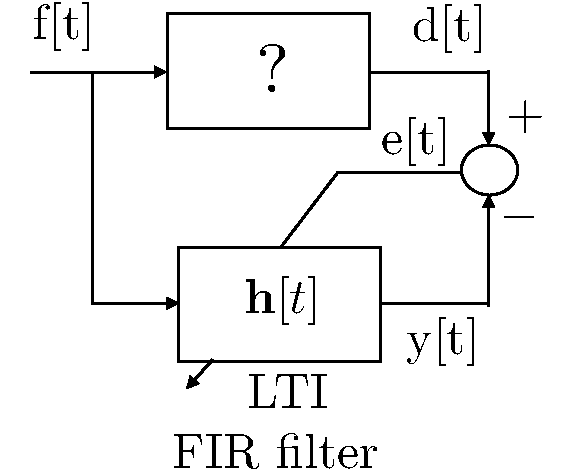
\includegraphics[width=0.5\textwidth]
			{figures/chap14_adaptive_filter}
	\end{center}
	Recall the RLS adaptive filter algorithm.
	
	The objective is to minimize the error
	\[ 
		J(\hbf) = (d[t] - y[t])^2.
	\]
	
	\begin{itemize}
		\item The RLS minimizes the squared error of all past outputs, but LMS only minimizes the squared error of the current output.
		\item The RLS algorithm was derived using the projection theorem.
		\item LMS is derived using gradient descent.
	\end{itemize}
\end{frame}

%----------------------------------
\begin{frame}\frametitle{LMS Adaptive Filtering}
	Assume that the output of the adaptive filter is
	\[ 
		y[t] = \sum_{\ell = 0}^{m-1}h[\ell]f[t-\ell] = \fbf^\top[t]\hbf
	\]
	where
	\[
		\fbf[t] 
			= \begin{pmatrix}
	    		f[t]\\
	    		f[t-1]\\
	    		\vdots\\
	    		f[t-m+1]
	  		  \end{pmatrix}
	  	\text{ and }
		\hbf
			= \begin{pmatrix}
	    		h[0]\\
	    		h[1]\\
	    		\vdots\\
	    		h[m-1]
	  		  \end{pmatrix}
	\]
\end{frame}

%----------------------------------
\begin{frame}\frametitle{LMS Adaptive Filtering}
	Then
	\begin{align*}
		J(\hbf) 
			&= (d[t] - y[t])^2 \\
			&= (d[t] - \fbf^\top[t]\hbf)^2\\
			&= d^2[t] - d[t]\fbf^\top[t]\hbf - d[t]\hbf^\top f[t] + \hbf\fbf[t]\fbf^\top[t]\hbf
	\end{align*}
	where 
	\[ 
		\frac{\partial J}{\partial \hbf} 
			= 2\fbf[t]\fbf^\top[t] \hbf - 2d[t]\fbf[t] 
	\]
\end{frame}

%----------------------------------
\begin{frame}\frametitle{LMS Adaptive Filtering}
	So let
	\[ 
		\hbf[t+1] = \hbf[t] - \alpha \frac{\partial J}{\partial \hbf}(\hbf[t]) 
	\]
	gives
	\begin{align*}
		 \hbf[t+1] 
		 	&= \hbf[t] - 2\alpha(\fbf[t]\fbf^\top[t]\hbf[t] - d[t]\fbf[t])\\
			&= \hbf[t] + \mu \fbf[t](d[t] - \fbf^\top[t]\hbf[t])\\
	\end{align*}
	\[
		\fbox{$\hbf[t+1] = \hbf[t] + \mu \fbf[t]e[t]$}
	\]
	This is known as the LMS adaptive filter.
	
	\vfill
	
	Compare to RLS...
	
	For discussion on convergence, consult Moon Chap~14...
\end{frame}

%%----------------------------------
%\begin{frame}\frametitle{LMS Adaptive Filtering}
%	{\color{blue}Question:} Does the LMS algorithm converge?
%	
%	\vfill
%	
%	Since $J(\hbf)$ is quadratic, we suspect it might converge when
%	\[ 
%		0 < \mu < \frac{2}{\lambda_{\max(R)}}. 
%	\]
%	This is shown in the book under some bad assumptions.	
%	Since we don't know $R$ we can proceed as follows:
%	
%	\[ 
%		tr(R) = \sum_{j=1}^m\lambda_j 
%	\]
%	so
%	\[ 
%		\lambda_{\max(R)} \leq \sum_{j=1}^m\lambda_j  \qquad (\lambda_j > 0) 
%	\]
%\end{frame}
%
%%----------------------------------
%\begin{frame}\frametitle{LMS Adaptive Filtering}
%	But
%	\begin{align*}
%		R 
%			&= E\{f[t]f^T[t]\}\\
%			&= E\left\{ 
%					\begin{pmatrix}
%			       		f[t]\\
%			       		f[t-1]\\
%			       		\vdots\\
%			       		f[t-m+1]
%			      	\end{pmatrix}
%			      	\begin{pmatrix}
%			    		f[t] & \cdots & f[t-m+1]
%			  		\end{pmatrix} 
%		  		\right\}\\
%			&= E\left\{ 
%		      		\begin{pmatrix}
%		       			f[t]f[t]\\
%		       			& f[t-1]f[t-1]\\
%		       			& & \ddots\\
%		       			& & & f[t-m+1]f[t-m+1]
%		      		\end{pmatrix}
%				\right\}
%	\end{align*}
%	
%	If $f$ is a random variable with variance $\sigma^2$ then $tr(R) = m\sigma^2$ so if 
%	\[
%		0 < \mu < \frac{2}{m\sigma^2} < \frac{2}{m\lambda_{\max(R)}}
%	\]
%	then LMS converges.	
%\end{frame}



\end{document}